%%%%%%%%%%%%%%%%%%%%%%%%%%%%%%%%%%%%%%%%%%%%%%%%%%%%%%%%%%%%%%%%%%%%%%%%%
%%   CHAPTER: THE 0E0P METACELL
%%%%%%%%%%%%%%%%%%%%%%%%%%%%%%%%%%%%%%%%%%%%%%%%%%%%%%%%%%%%%%%%%%%%%%%%%

\renewcommand{\chapterfolder}{0e0p/}
\chapterimage{cover/0e0p}
\chapter{The 0E0P Metacell}\label{chp:0e0p}\index{0E0P metacell}


\vspace*{-0.4in}
\epigraph{If you couldn't predict what [Life] did then probably that's because it's capable of doing anything.}{John H. Conway}
\vspace*{0.15in}


\noindent In the previous chapter, we introduced universal construction and presented several adjustable spaceships based on it. In this chapter, we explore a more complex application of universal construction: a self-reproducing pattern that interacts with nearby copies of itself so as to emulate Conway's Game of Life, or a different cellular automaton, on a much larger and slower scale.

Specifically, we construct a pattern called the \textbf{0E0P metacell},\footnote{Constructed by Adam P.~Goucher from 2014 to November 2018. The acronym ``0E0P'' stands for ``(State) 0 Encoded by 0 Population'', in reference to the fact that its ``off'' state is just a metacell-sized region of empty space---its most remarkable property, which is not shared by any metacell that came before it (see Section~\ref{sec:0e0p_history}).} which has the property that if we arrange copies of it on the Life plane then, at a zoomed-out macroscopic scale, it evolves in the same way that the corresponding arrangement of cells would evolve. For example, if we place five copies of this metacell in the Life plane in the formation of a glider, as illustrated in Figure~\ref{fig:0e0p_glider}, then we indeed get a spaceship that travels like a glider (but much more slowly).

\begin{figure}[!htb]
	\centering
	\embedlink{0e0p_glider}{\vcenteredhbox{\patternimg{0.129}{0e0p_glider_0}} \vcenteredhbox{\color{black}{$\xrightarrow{\text{\clock{4}{45} $2^{36}$}}$}} \vcenteredhbox{\patternimg{0.129}{0e0p_glider_236}}}
	\caption{A \textbf{metaglider}\index{metaglider} made up of five copies of the 0E0P metacell, each of which is $2^{18} \times 2^{18}$ and logically makes up one ``cell''. It travels in much the same way as a glider, but $2^{36}$ times as slowly.}\label{fig:0e0p_glider}
\end{figure}

A meta-fied pattern like this is roughly $2^{18} = 262{\thousep}144$ times as large as the original pattern that it is based on, and it runs $2^{36} = 68{\thousep}719{\thousep}476{\thousep}736$ times as slowly. Indeed, the 0E0P metacell is so much larger and slower than any other pattern that we have seen in this book that evolving the metaglider from Figure~\ref{fig:0e0p_glider} through four ``metagenerations'' (i.e., $4 \times 2^{36}$ generations), to see that it really is a spaceship, would take a couple of years on a modern desktop computer via standard Life simulation algorithms.\footnote{The fastest ``standard'' Life simulation algorithm is \textbf{HashLife} \cite{Gos84}, which is fast enough to run any of the patterns that we saw earlier in this book---even huge ones like the $\pi$ calculator of Section~\ref{sec:pi_calc} and the Gemini spaceship of Section~\ref{sec:gemini_itself}. To run patterns that use huge streams of gliders (like the 0E0P metacell) more efficiently, Adam P.~Goucher developed a new \textbf{StreamLife} algorithm, but even it would require several months to evolve a metaglider through four metagenerations.}\index{HashLife}\index{StreamLife}

While emulating Life within Life perhaps does not seem as remarkable a feat as some of the other things we have achieved over the past three chapters, what really makes the 0E0P metacell shine is that it can actually emulate a huge variety of 2D cellular automata besides Life as well. As a result, any pattern from one of those other cellular automata can be straightforwardly ``imported'' into Life simply by meta-fying it, thus giving us exotic new types of patterns that were previously not known how to construct.

To illustrate this phenomenon, consider the cellular automaton that has all the same rules as Life, plus the additional rule that a dead cell comes to life if it has exactly $6$ live neighbors (i.e., the Life-like cellular automaton with rulestring\index{rulestring} B36/S23). This cellular automaton is called \textbf{HighLife},\index{HighLife} and it is interesting for the fact that it has a simple \textbf{replicator}:\index{replicator (pattern)} a pattern that produces arbitrarily many copies of itself, as illustrated in Figure~\ref{fig:highlife_replicator}.

\begin{figure}[!htb]
	\centering
	\embedlink{highlife_replicator}{\vcenteredhbox{\patternimg{0.122}{highlife_replicator_0}} \vcenteredhbox{\genarrow{12}} \vcenteredhbox{\patternimg{0.122}{highlife_replicator_12}} \vcenteredhbox{\genarrow{12}} \vcenteredhbox{\patternimg{0.122}{highlife_replicator_24}} \vcenteredhbox{\genarrow{12}} \vcenteredhbox{\patternimg{0.122}{highlife_replicator_36}}}
	\caption{A \textbf{replicator} in the HighLife (B36/S23) Life-like cellular automaton that duplicates itself every $12$~generations. This replicator (and HighLife itself) was found by Nathan Thompson in 1994.}\label{fig:highlife_replicator}
\end{figure}

After this replicator copies itself the first time, each of its copies attempt to do the same. However, since these copies are right next to each other, two of \emph{their} copies attempt to occupy the same space, and instead annihilate each other (while their other copies are successfully created farther away). This behavior repeats forever: every $12$~generations, if there is space for a copy of this replicator then it is made, but two copies being made at the same spot at the same time mutually annihilate. The result is that after $n$ replication cycles (i.e., at generation $12n$), the sequence of replicators corresponds to the binary representation of $n$ (with a ``1'' being represented by the presence of a copy of the replicator, and a ``0'' being represented by empty space), followed by its mirror-image.

Since we're using HighLife's rules that require birth when a dead cell has $6$ live neighbors, this is not a valid replicator in Life: when run, it merely degenerates into a configuration of eight blinkers. However, we can ``import'' its behavior into regular Life by programming the 0E0P metacell to emulate HighLife and then arranging $12$ copies of that metacell in the same formation as the $12$~cells that make up the replicator from Figure~\ref{fig:highlife_replicator}. This meta-fied replicator is displayed in Figure~\ref{fig:meta_replicator}.\footnote{Slsparse (see \httpsurl{conwaylife.com/wiki/Slsparse}) comes with a Python script called \texttt{isotropic\_metafier.py} that can metafy patterns like this automatically.} While it is not the first replicator to be constructed in Life (that honor goes to the linear propagator\index{linear propagator} that we mentioned in Section~\ref{sec:universal_construction_history}), this is just the tip of the monumental iceberg of what can be done with the 0E0P metacell.

\begin{figure}[!htb]
	\centering
	\embedlink{metareplicator}{\vcenteredhbox{\patternimg{0.135}{metareplicator_0}} \vcenteredhbox{\color{black}{$\xrightarrow{\text{\clock{4}{55} $12 \times 2^{36}$}}$}} \vcenteredhbox{\patternimg{0.135}{metareplicator_12}}}
	\caption{A replicator in Conway's Game of Life that is made up of twelve 0E0P metacells, each emulating the HighLife rule (B36/S23) from Figure~\ref{fig:highlife_replicator}.}\label{fig:meta_replicator}
\end{figure}

In this chapter, we first explore a few other cellular automata that have exotic patterns that can be implemented in this way in Life via the 0E0P metacell, and then we describe the inner workings of the 0E0P metacell itself.


%%%%%%%%%%%%%%%%%%%%%%%%
\section{Other 2D Cellular Automata}\label{sec:other_ca_rules}
%%%%%%%%%%%%%%%%%%%%%%%%

While cellular automata can act on grids of any dimension and of a variety of different shapes, all of the ones that we consider (and all of the ones that can be emulated by the 0E0P metacell) act on a 2-dimensional square grid. Furthermore, for now we only consider cellular automata that use two states, which we still refer to as ``alive'' and ``dead'', and the Moore neighborhood of Figure~\ref{fig:neighborhood}, though we will see in Section~\ref{sec:0e0p_rule_emulation} that the 0E0P metacell can emulate some cellular automata without these two restrictions.


%%%%%%%%%%%%%%%%%%%%%%%%
\subsection{Life-Like (i.e., Outer-Totalistic) Cellular Automata}\label{sec:lifelike_rules}\index{Life-like}\index{outer-totalistic}\index{totalistic}
%%%%%%%%%%%%%%%%%%%%%%%%

A $2$-state cellular automaton is called \textbf{outer-totalistic} if the birth and death rules depend only on the state of the current cell, as well the number of live neighbors that it has.\footnote{In contrast with \textbf{totalistic} cellular automata, in which the birth and death rules depend only on the number of live neighbors including the cell itself.} That is, they are exactly the cellular automata that can be described by the Bx/Sy rulestring\index{rulestring} notation that was introduced earlier. An outer-totalistic cellular automaton is said to be \textbf{Life-like} if it furthermore satisfies all of the properties that we assumed at the start of this section (i.e., it acts on a 2-dimensional square grid and neighbors are counted according to the Moore neighborhood).

Some Life-like cellular automata have simple patterns that behave unlike any simple patterns that are known in Life itself, as evidenced by the replicator that we saw in Figure~\ref{fig:highlife_replicator}. While that pattern replicates along a single line, there are also Life-like rules that give rise to simple replicators that replicate in multiple directions and fill the whole plane. In fact, in the appropriately-named \textbf{replicator}\index{replicator (rule)} rule (B1357/S1357), \emph{every} pattern is a replicator that repeatedly produces copies of itself in all $8$ orthogonal and diagonal directions---see Figure~\ref{fig:replicator_smile}.

\begin{figure}[!htb]
	\centering
	\embedlink{replicator_smile}{\vcenteredhbox{\patternimg{0.25}{replicator_smile_0}} \vcenteredhbox{\genarrow{8}} \vcenteredhbox{\patternimg{0.11486486484}{replicator_smile_8}} \vcenteredhbox{\genarrow{8}} \vcenteredhbox{\patternimg{0.06789137379}{replicator_smile_16}} \vcenteredhbox{\genarrow{8}} \vcenteredhbox{\patternimg{0.0927947598}{replicator_smile_24}}}
	\caption{In the \textbf{replicator} rule (B1357/S1357), every pattern is a replicator that creates copies of itself in the $8$ standard directions.}\label{fig:replicator_smile}
\end{figure}

% Proof that replicator rule really does replicate in exercises? Maybe a 5/5 difficulty with a mild hint suggesting XOR?
% Maybe exercise: how long does it take for a pattern to replicate, as a function of its bounding box size? Solution: 2^(ceil(log_2(n))) generations for a pattern with longest side length n.

% https://www.conwaylife.com/forums/viewtopic.php?p=131063#p131063 (quad growth, spiral growth)


%%%%%%%%%%%%%%%%%%%%%%%%
\subsection{Isotropic (but Non-Totalistic) Cellular Automata}\label{sec:isotropic_rules}\index{isotropic}
%%%%%%%%%%%%%%%%%%%%%%%%

Stuff.
% Isotropic (contains outer-totalistic): invariant under rotations and reflections
% https://www.conwaylife.com/wiki/Isotropic_non-totalistic_Life-like_cellular_automaton
% T-tet SMOS goes here
% RRO goes here too: https://conwaylife.com/wiki/Reflectorless_rotating_oscillator
% There is *lamost* one in a Life-like, but just give a footnote/exercise about it. Exercise could ask why it's not a true RRO.


%%%%%%%%%%%%%%%%%%%%%%%%
\subsection{Non-Isotropic Cellular Automata}\label{sec:non_isotropic_rules}\index{non-isotropic}
%%%%%%%%%%%%%%%%%%%%%%%%

Stuff.
% Single-cell oblique spaceship in a non-isotropic rule: https://www.conwaylife.com/forums/viewtopic.php?f=11&t=3089&p=95700&hilit=MAP#p96359
% Maybe the c/714 single-cell?
% https://www.conwaylife.com/forums/viewtopic.php?f=11&t=3089&hilit=MAP&start=50#p98128

% Count number of rules, mention all can be emulated by 0E0P


%%%%%%%%%%%%%%%%%%%%%%%%
\section{Rule Emulation}\label{sec:0e0p_rule_emulation}
%%%%%%%%%%%%%%%%%%%%%%%%

Conway's Game of Life is a 2-state 9-neighbour rule: the next state of a cell
depends on the current state of the cell together with the current states of
the eight surrounding cells. Building a metacell that directly emulates Life
would be highly nontrivial for several reasons:\smallskip

% TODO: go back to earlier itemizes and add bold brief names like this one
\begin{itemize}
	\item \textbf{Quantity of neighbors}: each metacell would need to be able to
	construct a copy of itself in up to eight different positions. If both the
	north and east neighbours are present, it may be difficult to manoeuvre a
	construction arm to build the north-east neighbour.\smallskip
	
	\item \textbf{Survival}: a cell can live for multiple generations, so its
	logic circuitry would need to be reusable. Reusable circuitry is considerably
	more expensive than single-use circuitry: compare, for instance, the size of
	a boat and a Snark --- the smallest known single-use and reusable stable
	reflector, respectively.\smallskip
\end{itemize}

One of the main ideas behind the 0E0P metacell is that we can emulate any
2-state 9-neighbour rule with an 8-state 4-neighbour rule, where a cell
$(x, y)$ can only be alive at time $t$ if $x + y + t$ is even. This means
that whenever a cell is alive, all four neighbours are dead, so there is
plenty of empty space; moreover, every live cell always dies.

We use the cell states $\{ 0, 1, 2, 3, 4, 5, 6, 7 \}$, where the background
is state 0. In even generations in the emulating rule, the pattern consists
entirely of cells in states $\{ 0, 7 \}$; a live cell at position $(x, y)$
in generation $t$ of the original rule is encoded by a state-$7$ cell at
position $(x + y, y - x)$ in generation $2t$ of the emulating rule.

In odd generations, the pattern consists entirely of cells in states
$\{ 0, 1, 2, 3, 4, 5, 6 \}$. The transition rule for computing generation
$2t + 1$ from generation $2t$ is a fixed function:

$$ h : \{ 0, 7 \}^4 \rightarrow \{ 0, 1, 2, 3, 4, 5, 6 \} $$

specially chosen such that the following function is injective:

$$ H : \{ 0, 7 \}^9 \rightarrow \{ 0, 1, 2, 3, 4, 5, 6 \}^4 $$

% TODO ensure no page break between declaration and definition

$$ \begin{pmatrix}
a_{11} & a_{12} & a_{13} \\
a_{21} & a_{22} & a_{23} \\
a_{31} & a_{32} & a_{33}
\end{pmatrix} \mapsto \begin{pmatrix}
h(a_{11}, a_{12}, a_{21}, a_{22}) & h(a_{12}, a_{13}, a_{22}, a_{23}) \\
h(a_{21}, a_{22}, a_{31}, a_{32}) & h(a_{22}, a_{23}, a_{32}, a_{33})
\end{pmatrix} $$

Moreover, without loss of generality we can let $h(0, 0, 0, 0) = 0$.

The transition rule for computing generation $2t + 2$ from $2t + 1$ is a
function which depends on the rule being emulated:

$$ g : \{ 0, 1, 2, 3, 4, 5, 6 \}^4 \rightarrow \{ 0, 7 \} $$

The injectivity of $H$ means that we can specify the function $g$
such that the composition $g \circ H$ is exactly the transition rule
we want to emulate (up to having renamed the cell states to `0' and `7').
Making the necessary assumption that a dead cell surrounded entirely by
dead cells remains dead, we have $g(0, 0, 0, 0) = 0$. Consequently, we
can define a function:

$$ f : \{ 0, 1, 2, 3, 4, 5, 6, 7 \}^4 \rightarrow
\{0, 1, 2, 3, 4, 5, 6, 7 \} $$

where $f$ coincides with $g$ on the domain of $g$ and coincides with $h$
on the domain of $h$.

% TODO add an exercise to find a suitable function $h$. Up to permuting
% the different cell states, there are 200 different such functions.

The 0E0P metacell can be programmed to emulate any of the $8^{8^4-1}$
zero-preserving 8-state 4-neighbour rules. It takes $2^{35}$ generations
for the 0E0P metacell to run one generation of the 8-state rule (emulated
at a 45-degree angle), and therefore $2^{36}$ generations to emulate one
generation of the 2-state 9-neighbour rule (in the usual orientation).

% Explicitly state the 4-neighbor rule that emulates Life


%%%%%%%%%%%%%%%%%%%%%%%%%%%%%%%%%%%
\section{Structure of the Metacell}
%%%%%%%%%%%%%%%%%%%%%%%%%%%%%%%%%%%

\begin{figure}[htb]
	\centering
	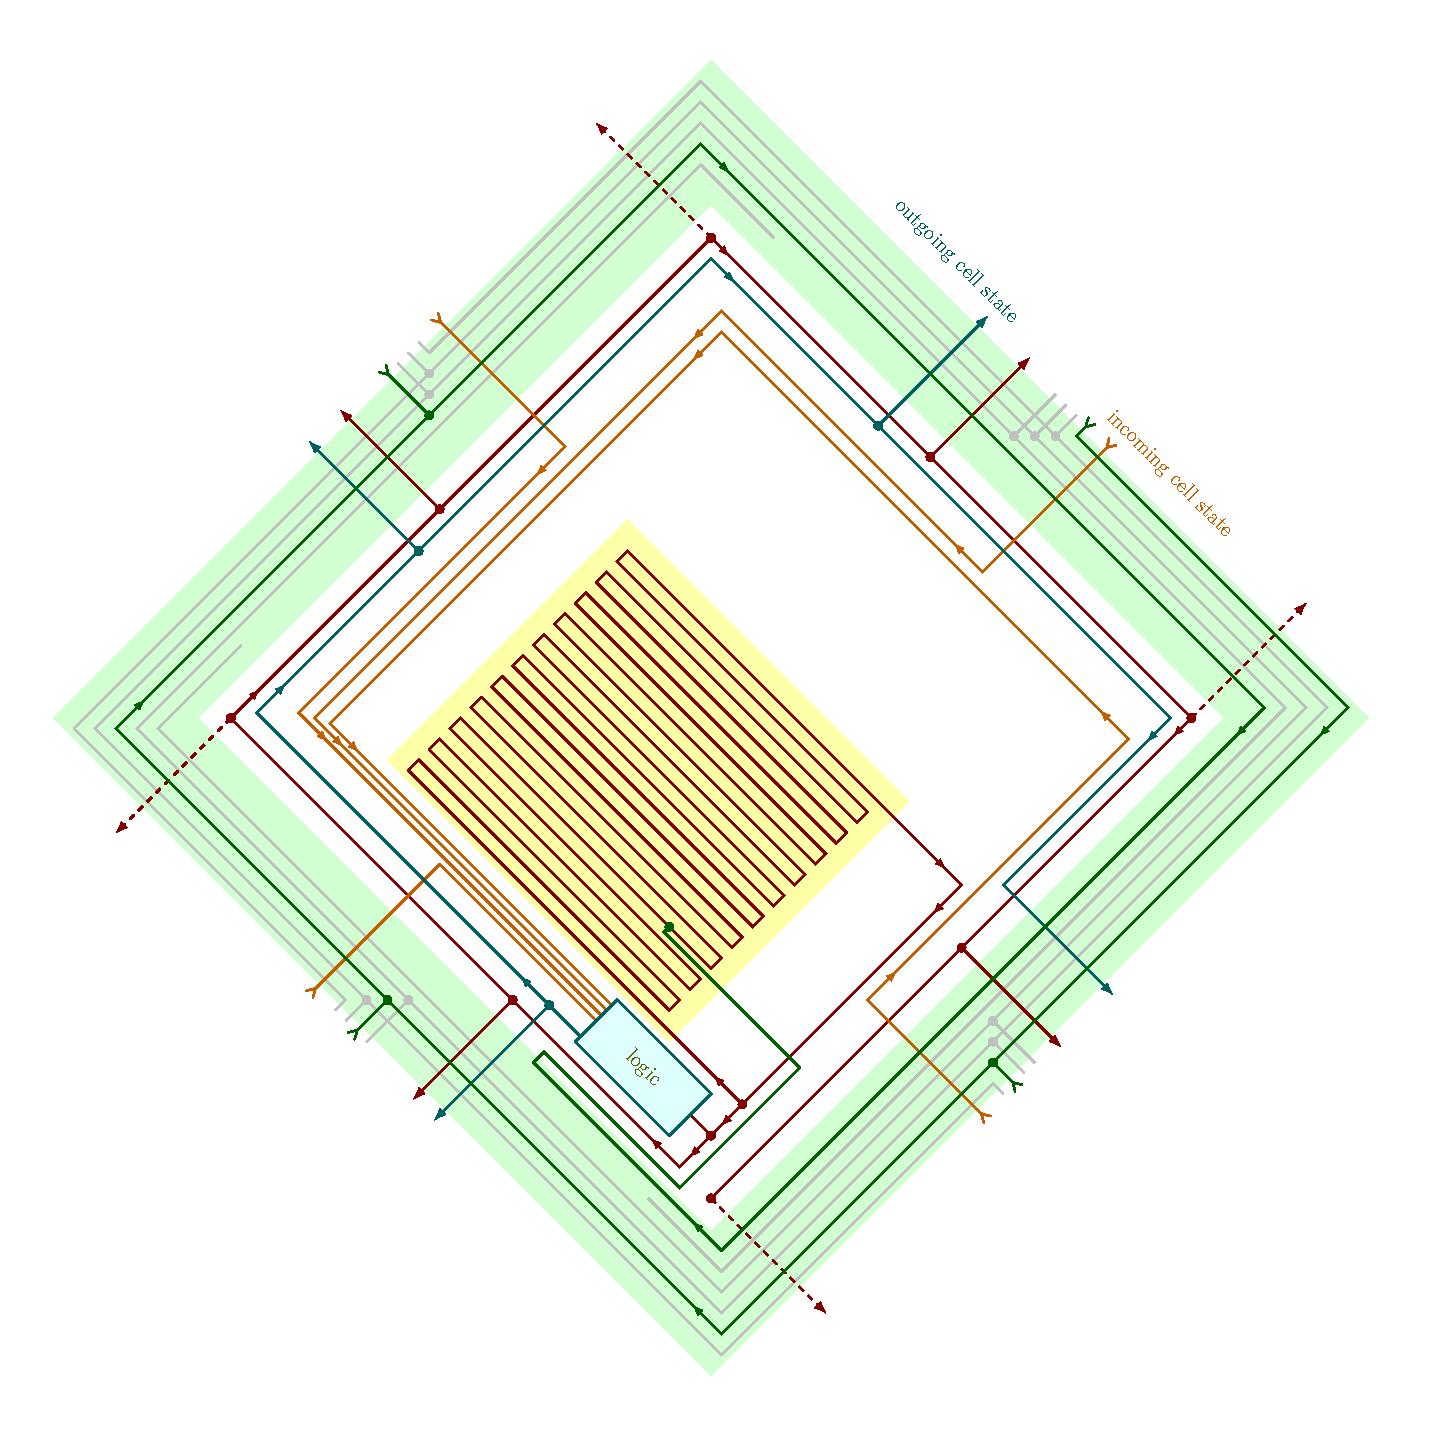
\includegraphics[width=\textwidth]{0e0p/0e0p_schematic.pdf}
	\caption{A schematic for the 0E0P metacell. The symmetrical outer
		\textbf{shell} is highlighted in pastel green, and the \textbf{nucleus}
		is highlighted in yellow. The unhighlighted region between them is the
		\textbf{kernel}.}\label{fig:0e0p_schematic}
\end{figure}

The large-scale structure of the metacell is tripartite, and each of the
three parts is constructed separately. The outer \textbf{shell} has exact
order-4 rotational symmetry, consisting of four spiral arms which propagate
gliders inwards. Only one of these arms is actually used; the other four
exist only to enforce the strict symmetry.

Inside the shell is the \textbf{kernel}, which does not have any symmetry
constraints. The south corner of the kernel contains logic circuitry for
regulating the metacell's lifecycle and computing the state of the metacell
based on the inputs from the four neighbouring cells. The kernel also contains
an output path, shown in crimson in Figure~\ref{fig:0e0p_schematic}, which
can connect to one of the four construction arms (violet, dashed) or to the
input spiral arm of one of the four neighbours. During the operation of the
metacell, the glider stream is redirected between the different possible
outputs by deleting Snarks.

The largest region of the metacell is the \textbf{nucleus}, a huge
boustrophedonic glider loop with a period of exactly $2^{29}$. The nucleus
is populated by over three million gliders, which together encode all of
the construction recipes along with the lookup table for the metacell's rule.

%%%%%%%%%%%%%%%%%%%%%
\section{Memory Tape}
%%%%%%%%%%%%%%%%%%%%%

Stuff.

%%%%%%%%%%%%%%%%%%%%%%%%%
\section{Logic Circuitry}
%%%%%%%%%%%%%%%%%%%%%%%%%

Stuff.

%%%%%%%%%%%%%%%%%%%%%%
\section{Construction}
%%%%%%%%%%%%%%%%%%%%%%

Stuff.


%%%%%%%%%%%%%%%%%%%%%%%%%%%%%%%%
\section{Notes and Historical Remarks}\label{sec:0e0p_history}\index{metacell}
%%%%%%%%%%%%%%%%%%%%%%%%%%%%%%%%

Many metacells---patterns of size larger than $1 \times 1$ that emulate the behavior of a single cell---were constructed prior to 0E0P. The first one was the \textbf{p5760~metacell}, which was constructed by David Bell in January 1996. This metacell is much smaller and faster than 0E0P, with a period of just $5760$~generations and a bounding box size of just $500 \times 500$ (see Figure~\ref{fig:p5760_metacell}). However, there are numerous trade-offs that make this metacell less useful:\smallskip

\begin{figure}[!htb]
	\centering
	\begin{tikzpicture}
	\node[inner sep=0pt,anchor=south west] at (0,0) {\embedlink{p5760_metacell}{\patternimg{0.15}{p5760_metacell}}};
	
	\draw[white,line width=2.5pt,opacity=0.6](2.63,8.15) circle (0.2);
	\draw[redback2,line width=1pt](2.63,8.15) circle (0.2);
	\end{tikzpicture}
	\caption{The \emph{p$5760$~metacell}. Whether the cell is considered ``alive'' or ``dead'' is determined by the presence or absence of a glider at the location circled in \bgbox{redback}{red}. That glider, if present, is duplicated $8$ times and sent to its neighbors along the $8$ output paths highlighted in \bgbox{aquaback}{aqua}, signaling to them that it is alive. Similarly, neighboring alive cells send their signals to this one along the input paths highlighted in \bgbox{magentaback}{magenta}.}\label{fig:p5760_metacell}
\end{figure}

\begin{itemize}
	\item[1)] It is hard-wired to emulate Life, and cannot easily be modified to emulate most of the $2^{512}$ different non-isotropic Life-like cellular automata.\smallskip
	
	\item[2)] It is not easy to tell at a glance which ``cells'' are alive and which are dead---it is determined by the presence or absence of a single extra glider in the cell---and thus is not interesting to look at from a far-out zoom level.\smallskip
	
	\item[3)] ``Dead'' cells must be placed on the Life plane, which means that, for example, spaceships cannot be emulated by this metacell unless the pattern is infinitely large.\smallskip
\end{itemize}

The first two of these problems were solved by the \emph{OTCA metapixel},\index{OTCA metapixel} which was constructed by Brice Due from late 2005 to mid-2006. While this metacell is a bit larger and slower than the first metacell (it is $2048 \times 2048$ and has period $35{\thousep}328$), it can be used to emulate any of the $2^{18}$ different outer-totalistic Life-like cellular automata. Indeed, built into its circuitry is an easily-adjustable array of eaters that determine how many live neighboring OTCA metapixels should lead to the birth or survival of the current metapixel (see Figure~\ref{fig:otca_metapixel}). 
% Introduce Life-like CA, since no introduction earlier
% mention out of the blue/honey bit/demultiplexer?

% FIGURE HERE, SHOWING PIXEL AND RULE ENCODINGS

The OTCA metapixel also has the remarkable feature that its alive and dead states look, from a distance, like alive and dead cells. This feature is achieved by the ``alive'' version of the cell releasing $43$ pairs of perpendicular lightweight spaceship streams that mutually annihilate each other, thus partially filling in the otherwise empty center of the metacell. For example, arranging a $1 \times 3$ row of ``alive'' metapixels (and a suitably large ``dead'' array of metapixels around its edges) results in a pattern that looks and evolves like a blinker, but $2{\thousep}048$ times as long and wide and $35{\thousep}328$ times as slow (see Figure~\ref{fig:metablinker}).

\begin{figure}[!htb]
	\centering
	\embedlink{metablinker}{\vcenteredhbox{\patternimg{0.104}{metablinker_0}} \vcenteredhbox{\color{black}{$\xrightarrow{\text{\clock{5}{46} 35328}}$}} \vcenteredhbox{\patternimg{0.104}{metablinker_35328}}}
	\caption{A \emph{metablinker}: an arrangement of OTCA metapixels that emulates a blinker, but with period $2 \times 35{\thousep}328$.}\label{fig:metablinker}\index{metablinker}
\end{figure}

The next notable metacell to be constructed was the \emph{p1 megacell},\index{p1 megacell} by Adam P.~Goucher in 2008. This metacell was, again, larger and slower than the metacells that came before it, with a bounding box of $2^{15} \times 2^{15}$ and a period of $2^{24}$. The new features this time that warranted the extra size and delay were twofold:\smallskip

\begin{itemize}
	\item This metacell was built entirely out of stable (p$1$) components like Herschel tracks, with the exception of a single period~$2^{24}$ gun used to regulate its timing.\footnote{This gun could be swapped out for a gun of another period, but periods that are multiples of $2$ help the pattern run quicker under the HashLife algorithm in Life simulation software like Golly.}\index{HashLife}\smallskip
	
	\item All $2^{512}$ non-totalistic Life-like cellular automata can be emulated by this metacell, versus the $2^{18}$ outer-totalistic Life-like cellular automata that can be emulated by the OTCA metapixel.\smallskip
\end{itemize}

% Figure of p1 megacell? Have had a lot of big figures bunched up closely here, so maybe not.

Finally, Adam P.~Goucher spent 2014--2018 constructing the 0E0P metapixel, which solved problem~(3) described earlier---it does not require a background grid of ``dead'' cells to be placed on the Life plane.

%https://www.conwaylife.com/forums/viewtopic.php?f=15&t=4117#p82954
%https://cp4space.hatsya.com/2018/11/12/fully-self-directed-replication/
%https://www.conwaylife.com/forums/viewtopic.php?f=2&t=3835
%https://www.conwaylife.com/forums/viewtopic.php?t=3968

% EXERCISE: Give reactions in HighLife-replicator-ship.rle from Golly and ask reader to make ship out of it


%%%%%%%%%%%%%%%%%%%%%%%%%%%%%%%%%
\section*{Exercises \hfill \normalfont\textsf{\small solutions to starred exercises on \hyperlink{solutions_0e0p}{page \pageref{solutions_0e0p}}}}
\label{sec:solutions_0e0p}
\addcontentsline{toc}{section}{Exercises}
\vspace*{-0.4cm}\hrulefill\vspace*{-0.3cm}\footnotesize\begin{multicols}{2}\vspace*{-0.4cm}\raggedcolumns\interlinepenalty=10000
	\setlength{\parskip}{0pt}
	%%%%%%%%%%%%%%%%%%%%%%%%%%%%%%%%%
	
	
	\begin{problem}\label{exer:0e0p_hamming_weight} \probdiff{1}
		Construct a formula for the population of the replicator from Figure~\ref{fig:highlife_replicator} in generation $12n$, where $n \geq 0$ is an integer. You may use the \emph{Hamming weight}\index{Hamming weight} of $n$, denoted by $H(n)$, which counts the number of ``1'' bits in the binary representation of $n$.
	\end{problem}
	
	
	\mfilbreak
	
	
	\begin{problem}\label{exer:0e0p_ex2}
		Another exercise could be placed here.
	\end{problem}
	
	
	%% EXERCISE END COMMANDS
\end{multicols}
\normalsize\vspace*{0.01cm}
%% DONE EXERCISE END COMMANDS
